\begin{description}
	\item[computational origami] \label{dictionary:computational-origami} -- a recent branch of computer science studying efficient algorithms for solving paper-folding problems.\cite{recent-results-in-computational-origami:paper}
	\item[crease] -- a line segment, along which a sheet of paper folds.
	\item[crease pattern] \label{dictionary:crease-pattern} -- a pattern of lines formed by creases that is created after unfolding the origami flat. For an example see figure \ref{fig:creasepattern}.
	\item[folded state] \label{dictionary:folded-state} -- An assembled origami model. Or alternatively, a sheet of paper folded along the crease pattern.
	\item[mountain] -- a fold of paper along the crease, such that the facets on the sides of the crease are facing downwards.
					\begin{figure}[H]
						\caption{Example of a mountain crease}
						\centering
						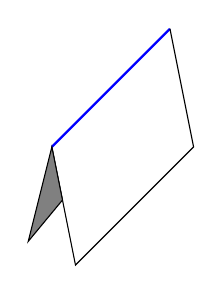
\begin{tikzpicture}[scale=1.5]
							\draw[blue, thick] (0,0) -- (1,1);
							\draw (1,1) -- (1.2, 0) --  (0.2, -1) -- (0,0);
							\filldraw[fill=gray] (0, 0) -- (-0.2, -0.8) -- (0.09, -0.45) -- cycle;
						\end{tikzpicture}
					\end{figure}
	\item[valley] -- A fold of paper along a crease, such that the facets on the sides of the crease are facing upwards.
					\begin{figure}[H]
						\caption{Example of a valley crease}
						\centering
						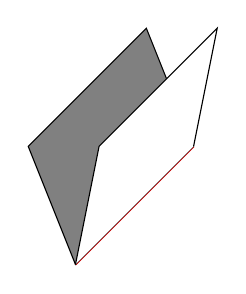
\begin{tikzpicture}[scale=1.5]
							\draw[red, thick] (0,0) -- (1,1);
							\filldraw[fill=gray] (0, 0) -- (-0.4, 1) -- (0.6, 2) -- (1, 1) -- cycle;
							\filldraw[fill=white] (1,1) -- (1.2, 2) --  (0.2, 1) -- (0,0);
						\end{tikzpicture}
					\end{figure}
	\item[mountain-valley assignment] -- an assignment of mountain or valley to the creases on the crease pattern.
	\item[.fold file] -- a file that conforms to the FOLD\cite{fold:paper} specification.
	\item[Instruction] -- a \textit{.fold} file created by a user, representing a sequence of steps required to
		fold a sheet of paper into a complete origami figure.
	\item[Transition] -- a folding animation played between two steps.
	\item[Guide] -- a set of all Transitions derived from an Instruction. Can be represented using a \textit{.fold} file.
	\item[Model] -- 3D representation of an origami figure. 
	\item[FPS] -- frames per second.
	\item[target angle] -- the supplement of the dihedral angle between the two neighbouring faces,
		towards which the faces should fold.
\end{description}

